% Created 2018-04-29 Sun 16:06
% Intended LaTeX compiler: pdflatex
\documentclass[10pt]{beamer}
\usepackage[utf8]{inputenc}
\usepackage[T1]{fontenc}
\usepackage{graphicx}
\usepackage{grffile}
\usepackage{longtable}
\usepackage{wrapfig}
\usepackage{rotating}
\usepackage[normalem]{ulem}
\usepackage{amsmath}
\usepackage{textcomp}
\usepackage{amssymb}
\usepackage{capt-of}
\usepackage{hyperref}
\usetheme{Boadilla}
\author{ECON 420: Game Theory}
\date{Spring 2018}
\title{Mixed Games}
\usecolortheme{seagull}
\usefonttheme[onlylarge]{structurebold}
\usefonttheme[onlymath]{serif}
\setbeamerfont*{frametitle}{size=\normalsize,series=\bfseries}
\setbeamertemplate{navigation symbols}{}
\setbeamertemplate{itemize item}[triangle]
\setbeamertemplate{footline}{}
\setbeamertemplate{enumerate items}[default]
\hypersetup{
 pdfauthor={ECON 420: Game Theory},
 pdftitle={Mixed Games},
 pdfkeywords={},
 pdfsubject={},
 pdfcreator={Emacs 25.2.2 (Org mode 9.1.6)}, 
 pdflang={English}}
\begin{document}

\maketitle

\begin{frame}[label={sec:org370fa88}]{}
\alert{Mixed simultaneous and sequential games}
\begin{itemize}
\item Real world games are often combinations of sequential and simultaneous games
\item We can use a combination of roll-back and best response analysis to find NE of these games
\end{itemize}
\end{frame}

\begin{frame}[label={sec:orgaefa102}]{}
\begin{center}
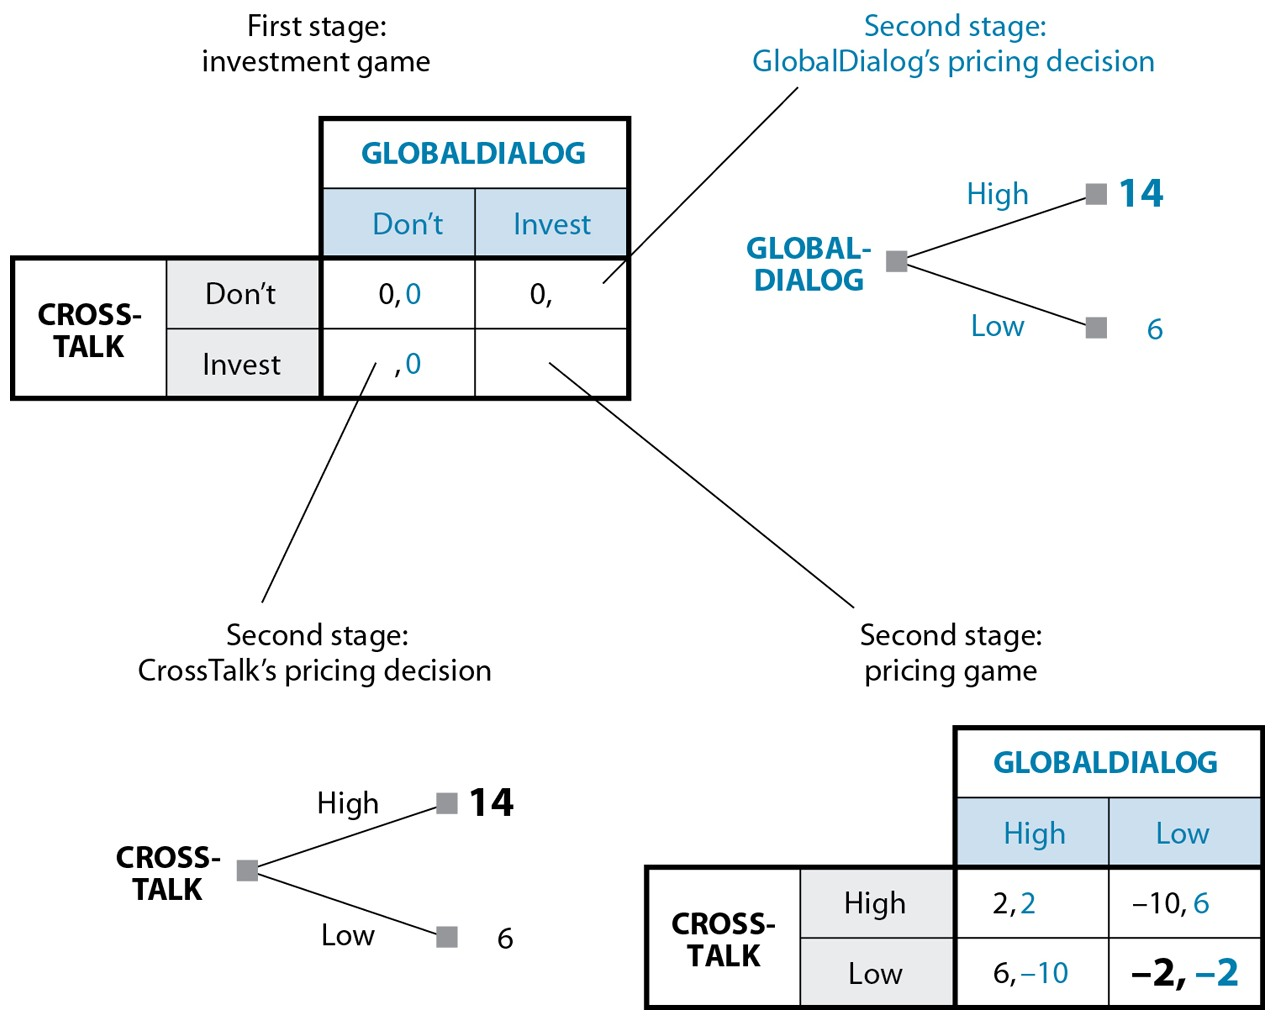
\includegraphics[width=.75\textwidth]{./img/GAMES4_FIG06.01.jpg}
\end{center}
\end{frame}

\begin{frame}[label={sec:orgf073e7b}]{}
\begin{center}
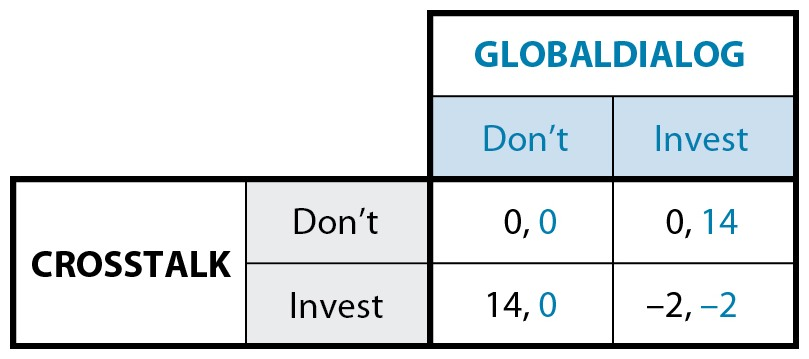
\includegraphics[width=.75\textwidth]{./img/GAMES4_FIG06.02.jpg}
\end{center}
\end{frame}
\begin{frame}[label={sec:orgf67990c}]{}
\begin{center}
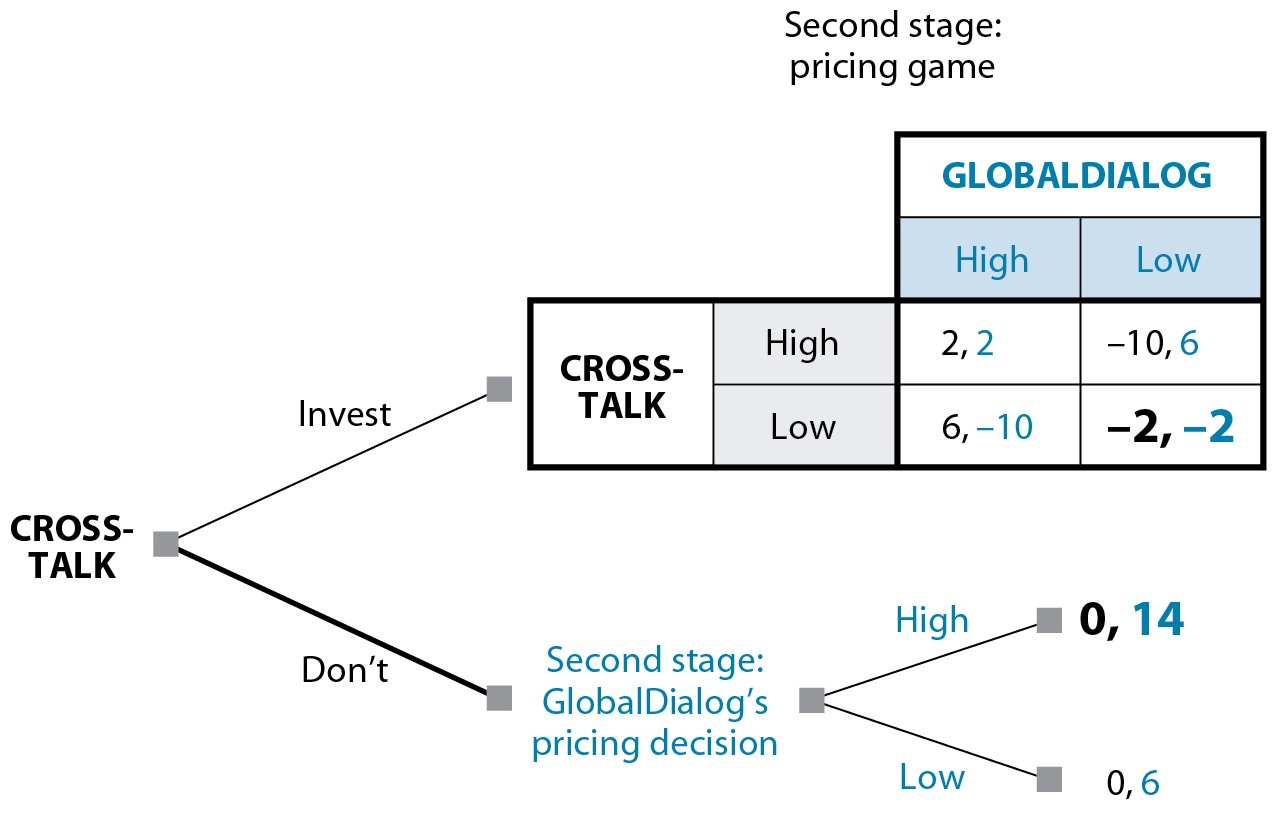
\includegraphics[width=.75\textwidth]{./img/GAMES4_FIG06.03.jpg}
\end{center}
\end{frame}

\begin{frame}[label={sec:org72f783f}]{}
\begin{center}
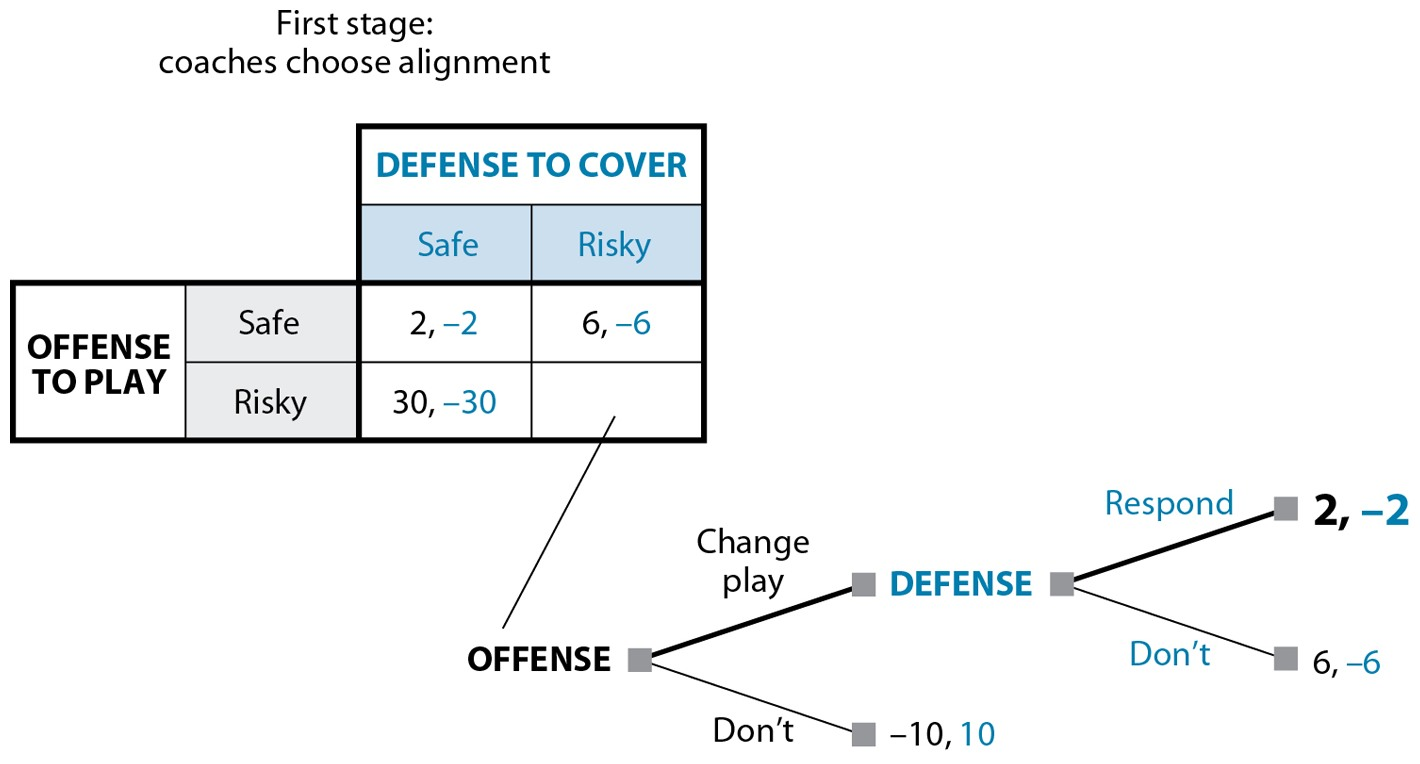
\includegraphics[width=.75\textwidth]{./img/GAMES4_FIG06.04.jpg}
\end{center}
\end{frame}

\begin{frame}[label={sec:org2c59a94}]{}
\alert{Simultaneous as sequential}
\begin{itemize}
\item Simultaneous games with multiple equilibria might have different outcomes if played sequentially (change the rules of the game)
\item Payoffs may be better for one of the players depending on move order
\begin{itemize}
\item First or second mover advantages
\end{itemize}
\end{itemize}
\end{frame}

\begin{frame}[label={sec:org9859aec}]{Example: Chicken (6.5)}
\end{frame}

\begin{frame}[label={sec:orge31e862}]{Example: Tennis (4.14)}
\end{frame}

\begin{frame}[label={sec:org2a3d191}]{Example: Monetary-Fiscal Policy Game (6.6a)}
\end{frame}

\begin{frame}[label={sec:org1a0aa76}]{}
\alert{Expressing simultaneous games in extensive form}
\begin{itemize}
\item Simultaneous-move games don't actually require players to move at the same time
\begin{itemize}
\item Players are simply unaware of what other player chooses when they make their choice
\end{itemize}
\item We can use \emph{information sets} to describe this situation in simultaneous games
\begin{itemize}
\item We draw a circle around nodes that are in the same information set
\item Players at a particular information set do not know which node they are at (within the set)
\end{itemize}
\end{itemize}
\end{frame}

\begin{frame}[label={sec:orge703de7}]{Example: Tennis (4.14)}
\end{frame}

\begin{frame}[label={sec:org1362e67}]{}
\alert{Expressing sequential games in normal form}
\begin{itemize}
\item Strategies are \emph{complete plans of action}
\item In a sequential game, this means we must describe the action of a player at \emph{any possible node} where they might move
\item This includes actions on \emph{off equilibrium paths}
\end{itemize}
\end{frame}

\begin{frame}[label={sec:orgcaabbb4}]{Example: Monetary-Fiscal Policy Game (6.6c)}
\end{frame}

\begin{frame}[label={sec:org80582fe}]{Subgame Perfect NE (SPNE)}
\begin{itemize}
\item Some NE are supported by \emph{threats} of actions that may not be \emph{credible} if the player is actually made to choose at that particular node
\item We can describe the NE outcomes that don't require threats as SPNE
\item A \emph{subgame} is any possible "mini game" that results after any path of play
\item The NE that are also NE for their respective subgames are SPNE
\end{itemize}
\end{frame}
\end{document}